\documentclass[12pt,a4paper]{article}
\usepackage[margin=2.4cm]{geometry}
\usepackage{fontspec}
\usepackage{graphicx}
\usepackage{booktabs}
\usepackage{amsmath,amssymb}
\usepackage{hyperref}
\usepackage{caption}
\usepackage{subcaption}
\usepackage{setspace}
\usepackage{xcolor}
\usepackage{float}
\setmainfont{Noto Serif CJK SC}
\setsansfont{Noto Sans CJK SC}
\XeTeXlinebreaklocale "zh"
\XeTeXlinebreakskip=0pt plus 1pt minus 0.1pt
\onehalfspacing
\hypersetup{colorlinks=true,linkcolor=black,citecolor=black,urlcolor=blue}
\captionsetup{font=small,labelfont=bf}
\renewcommand{\figurename}{图}
\renewcommand{\tablename}{表}
\renewcommand{\abstractname}{摘要}
\renewcommand{\refname}{参考文献}

\title{\textbf{超低信噪比条件下一次性 FPV 机群的涌现式瞄准}\\[0.35em]
\large 简单近邻规则与 Transformer 策略的仿真对比}
\author{战场仿真实验报告\\
\texttt{battlefield-sim} 平台}
\date{2026 年 8 月}

\begin{document}
\maketitle

\begin{abstract}
第一人称视角（FPV）自杀式无人机已经把单机成本压到消费电子量级，但其编队协同仍受两类硬约束支配：其一，超低空、强地杂波与电子对抗使机间无线电长期工作在 Shannon 容量接近零的超低信噪比区，能测到一个有效信息比特的到达时延已极为可贵；其二，一次性战斗部决定了为每架飞机配备 GPU/NPU 在费效上不合理。本文在可复现的二维圆形战场上对比两种\emph{仅使用本地 8+8 距离快照}的瞄准策略：作为研究目标的近邻涌现规则（最近合格目标严格近于最近友机才开火），以及作为机载人工智能对照的一层 Transformer 编码器（在 200 轮仿真上按目标平均存活时间相关的行为克隆训练）。杀伤区被构造为圆盘的外接正方形：6 条航线均分直径、探测半径等于航线间距，保证盘内任一点都被探测带覆盖。30 轮同种子评估表明，近邻规则的平均目标存活时间为 15.74\,s、场均中和 10.10 个目标；Transformer 为 15.79\,s 与 10.07 个。高斯配对检验不能拒绝效能相同（存活双侧 $p=0.239$），并在 $0.5\,\mathrm{s}$ 实务界内等效（TOST $p<10^{-12}$）；点估计上规则略优。规则每步 \texttt{compute\_ops} 约为 17，网络约为 $4.53\times 10^4$，相差约 2600 倍。结论是：在无法组网、不能摊销算力模组的一次性 FPV 上，基于测距的简单规则足以承担瞄准决策，把昂贵的神经网络放到每架机体上既无通信条件，也无费效依据。
\end{abstract}

\noindent\textbf{关键词：} FPV 自杀式无人机；超低信噪比；涌现智能；近邻规则；Transformer；机载算力费效

\section{引言}

消费级穿越机与开源飞控把“人在回路的单向攻击”变成了可规模化的一次性弹药。与巡飞弹或有人战机不同，这类平台有三个同时成立的特征：\textbf{单价极低}、\textbf{任务结束后机体销毁}、\textbf{只在视距/超低空无线电泡里短暂存活}。由此派生出两个经常被忽视的系统约束。

第一，机群几乎不能交换态势。超低空信道受地面反射、机体遮挡、敌方压制与同频模拟图传挤占，接收信噪比长期为负分贝。Shannon 公式\cite{shannon1948}
\begin{equation}
  C = B \log_2 (1+\mathrm{SNR})
\end{equation}
表明，当线性 $\mathrm{SNR}\ll 1$ 时 $C\approx B\cdot\mathrm{SNR}/\ln 2$，容量随信噪比坍缩\cite{sklar2001}。在此区间里，可靠地解码一个有效信息比特所付出的重传与时延，已经贵过该比特所能改变的战术决策。指望 12 架飞机在扫掠中共享目标清单或全局分配方案，是把有线数据链的假设错误地搬到了电子战环境。

第二，算力不能按“车载/机库”的逻辑摊销。一次性战斗部意味着 GPU 模组、散热、电池与软件维护成本都计入单发弹药。为每架 FPV 安装神经网络加速器，等价于把一枚便宜战斗部绑在一块不便宜的消费电子上，却换不来可复用的寿命。

这两条约束把问题从“如何训练更强的全局分配网络”收缩成：“在\emph{不能通信、不能上高算力}的前提下，本地简单规则能否达到与机载网络相当的杀伤效能？”本文用可复现仿真回答该问题。我们实现了圆形战场、外接矩形杀伤区、2 排$\times$6 架一次性 FPV 与 20 个静止假想敌；对比研究算法（近邻涌现规则）与对照算法（Transformer）。训练损失只使用目标平均存活时间所诱导的行为，计算耗时不进入 loss，仅作为硬件成本指标。

\section{相关约束与问题陈述}

\subsection{超低信噪比下的机间通信}

FPV 的典型载荷是模拟图传加窄带遥控。电子对抗条件下，可用带宽 $B$ 被压缩到数十 kHz 量级，且 $\mathrm{SNR}$ 可低于 $-10\,\mathrm{dB}$\cite{sklar2001}。以 $B=50\,\mathrm{kHz}$、$\mathrm{SNR}=-12\,\mathrm{dB}$（线性比 $10^{-1.2}$）为例，
\begin{equation}
  C = 5\times 10^{4}\cdot \log_2\!\bigl(1+10^{-1.2}\bigr) \approx 4.4\times 10^{3}\ \mathrm{bit/s}.
\end{equation}
若 12 机每秒广播 8 个目标距离（32 bit 浮点）加 8 个友机距离，原始载荷约 $12\times 16\times 32 = 6144$ bit，尚不含报头、校验与重传。这已经超过上述容量，更何况真实链路还要叠加突发误码与捕获时延。因此，\textbf{能测出一个有效信息的到达时刻本身就是稀缺资源}：任何依赖新鲜全局快照的分配算法，在物理层就已经迟到。

可行的信息通道只剩下两类：飞手到单机的上行（同样脆弱，且不能规模化到每机一名飞手），以及机体传感器对邻域的\emph{本地}测量（视觉、雷达、测距）。后者不经过无线电组网，时延是传感器帧周期而非 ARQ 时延。本文两种算法都只消费本地 8 条目标距离与 8 条友机距离，以符合该信道现实。

\subsection{一次性平台的算力经济学}

记单机出厂成本 $c_{\mathrm{air}}$、算力模组成本 $c_{\mathrm{npu}}$、任务成功概率 $p$。一次性使用下，摊销后的“每成功攻击算力开销”为 $c_{\mathrm{npu}}/p$，无法用飞行小时数稀释。微控制器完成十余次比较与一次最小值即可决策；神经网络即便是本文这种 $d_{\mathrm{model}}=16$ 的一层编码器，每次决策仍需约 $4.5\times 10^{4}$ 次乘加，若换成任务级视觉 Transformer 则再扩大数个数量级，并引入瓦级功耗与克级质量。对廉价自杀式弹药，这是错误的成本结构。

\subsection{研究问题}

在杀伤区完整覆盖圆形战场、每机至多保留 8+8 条距离、开火即消耗的前提下：

\begin{enumerate}
  \item 仅用最近友机距离与最近目标距离的三步规则，能否在目标平均存活时间上匹配一个经过 200 轮仿真训练的 Transformer？
  \item 二者的计算量（因而硬件成本）相差多少？
\end{enumerate}

若规则不差于网络而算力低三个数量级，则“给每架 FPV 装 AI 大脑”缺乏实验支持。

\section{仿真平台}

平台 \texttt{battlefield-sim} 以 Rust 实现，固定时间步 $\mathrm{d}t=0.01\,\mathrm{s}$，同一种子下除墙钟外完全可复现。源码与数据位于桌面工程目录。

\subsection{圆形战场与完美包含的矩形杀伤区}

战场是半径 $R=200\,\mathrm{m}$ 的闭圆盘，原点在圆心，$+Y$ 为扫掠方向。20 个假想敌按逆变换 $r=R\sqrt{u}$、$\,\theta=2\pi v$ 均匀洒在盘内。FPV 编为 2 排$\times$6 架，沿直径做包含端点的均分：
\begin{equation}
  x_i = -R + \frac{i}{5}\cdot 2R,\quad i=0,\ldots,5,
\end{equation}
即 $x\in\{-200,-120,-40,40,120,200\}$。相邻航线间距 $80\,\mathrm{m}$，横向最远点到最近航线 $40\,\mathrm{m}$。

所谓“矩形杀伤区宽度等于圆的直径”，在几何上就是圆盘的轴对齐外接正方形 $[-R,R]\times[-R,R]$：圆内切于该正方形。为使探测带把正方形的横向完全填满，取探测半径 $D=80\,\mathrm{m}$（等于航线间距）。相邻探测圆在中线处互相越过对方 $40\,\mathrm{m}$，因此 \textbf{盘内任意一点的横坐标必落入某架飞机的探测区间}；飞机沿 $+Y$ 匀速扫过 $y\in[-R-D,R+D]$ 后，纵坐标亦被覆盖。这就是杀伤区对圆形战场的完美包含：不是六条细线“碰巧擦过”，而是一条宽 $2R$ 的实心探测带把圆盘镶嵌其中。图~\ref{fig:field} 给出俯视示意。

\begin{figure}[H]
  \centering
  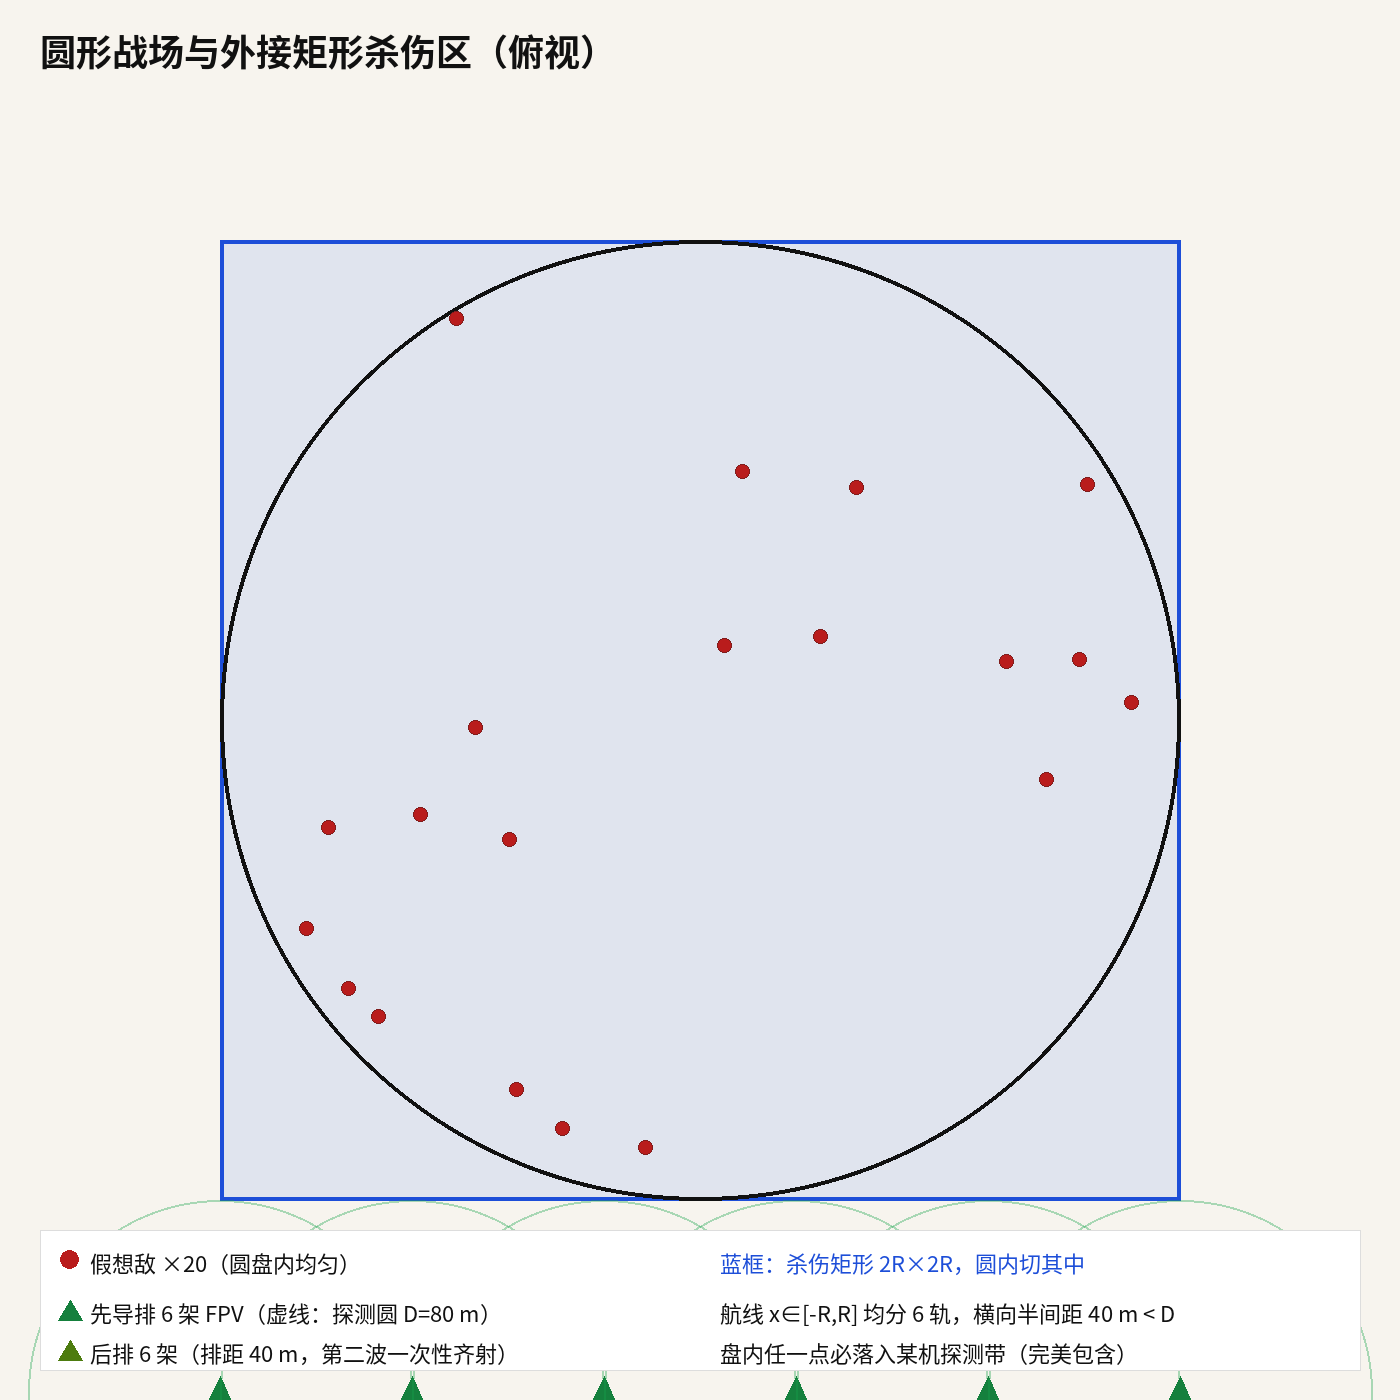
\includegraphics[width=0.92\textwidth]{figures/battlefield_schematic.png}
  \caption{圆形战场、外接矩形杀伤区、20 个假想敌与 2$\times$6 FPV 编队。先导排探测圆以虚线标出；$D=80\,\mathrm{m}$ 保证横向无盲区。}
  \label{fig:field}
\end{figure}

先导排从 $y=-R-D$ 出发，后排落后 $40\,\mathrm{m}$。速度 $v=25\,\mathrm{m/s}$。一次性消耗：完成 $T_{\mathrm{kill}}=0.05\,\mathrm{s}$ 的持续锁定后该机 \texttt{Expended}，不再射击。12 弹对 20 敌，未击中者在扫掠结束时刻 $T_{\mathrm{end}}$ 删失。评分
\begin{equation}
  \overline{T}_{\mathrm{surv}} = \frac{1}{20}\sum_{k=1}^{20} T_{\mathrm{surv}}^{(k)}
\end{equation}
计入全部目标；越小越好。计算量 \texttt{compute\_ops} 按公布的操作计数规则累加，\textbf{不进入训练损失}。

\subsection{本地传感}

每机每拍刷新最多 8 条最近敌距与 8 条最近友距（并列取更小 id）。记忆不过滤 $D$，但开火要求欧氏距离 $\le D$。同拍锁定对后续飞机的 \texttt{select} 输入保持陈旧，以避免隐式全局锁。该设定模拟的是“传感器帧”而不是“全知数据链”。

\section{两种算法}

二者输入完全相同：本地 $8+8$ 快照。差别只在决策函数。

\subsection{研究算法：近邻涌现规则}

图~\ref{fig:rule}。对合格目标（在 $D$ 内且未被其他机锁定）取最近距离 $d_{\mathrm{tgt}}$，对友机取最近距离 $d_{\mathrm{fr}}$。当且仅当
\begin{equation}
  d_{\mathrm{tgt}} < d_{\mathrm{fr}}
\end{equation}
时中和该最近目标，否则弃权。无友机时 $d_{\mathrm{fr}}=+\infty$，退化为就近开火。

\begin{figure}[H]
  \centering
  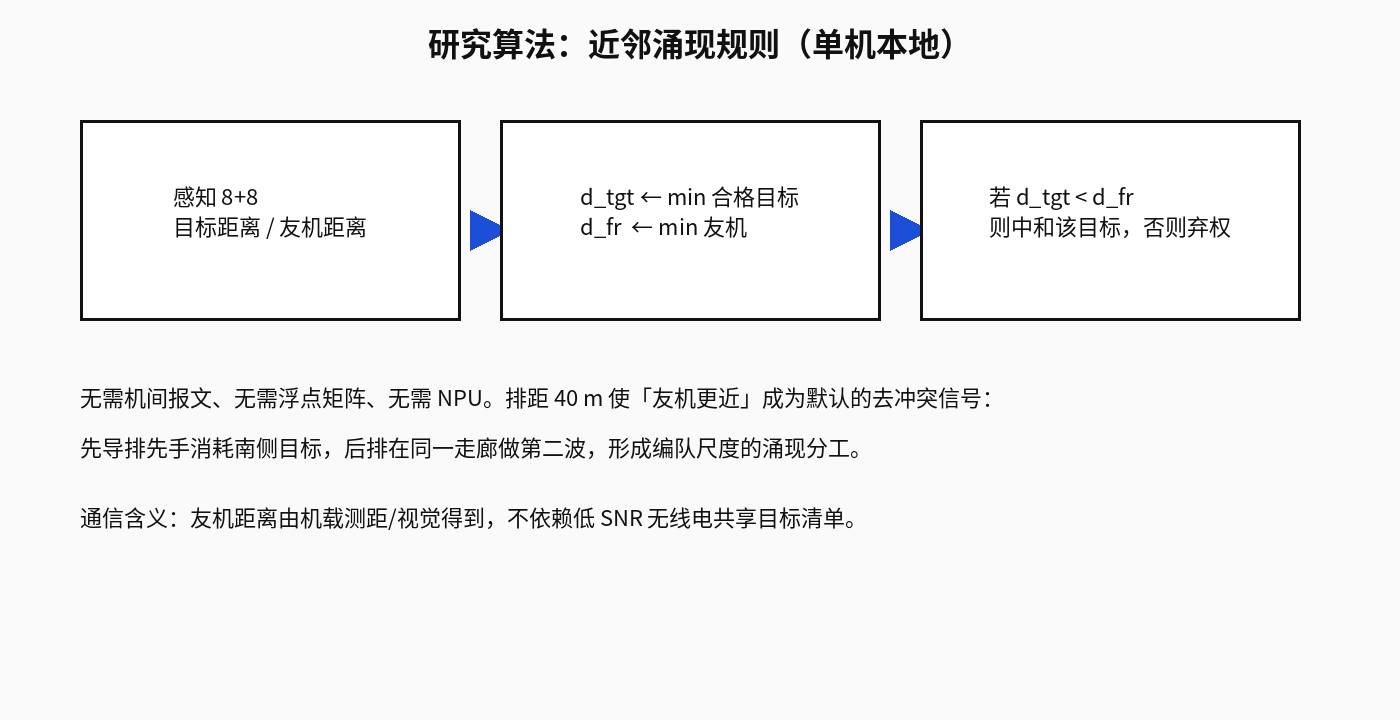
\includegraphics[width=0.92\textwidth]{figures/rule_flowchart.png}
  \caption{近邻涌现规则的三步本地决策。全程不发送机间报文。}
  \label{fig:rule}
\end{figure}

该规则的涌现性来自编队几何而非集中规划：同走廊上后排相对先导排约 $40\,\mathrm{m}$，故先导排在 $d_{\mathrm{tgt}}<40\,\mathrm{m}$ 时先手；先导消耗后，后排的“最近友机”消失或远离，第二波自然接替。横向 $80\,\mathrm{m}$ 间距大于 $D$ 的一半，邻轨抢夺被距离本身抑制。这是把物理编队写成了去冲突协议，与 Reynolds 的局部行为合成群体运动\cite{reynolds1987}、以及生物学中由局部规则产生宏观结构的自组织机制\cite{camazine2001}同一逻辑。

每步操作数：遍历友机与目标各一次、若干次最小值更新、一次比较，实验中均值约 17。

\subsection{对照算法：Transformer 瞄准网络}

网络将 CLS + 8 个目标 token + 8 个友机 token 送入一层双头编码器（$d_{\mathrm{model}}=16$，$d_{\mathrm{ff}}=32$），由 CLS 输出 9 维 logits（8 个目标槽 + 弃权）。架构取自 Vaswani 等提出的 Transformer 编码器块\cite{vaswani2017}，但宽度远小于原文翻译模型；这是“给每架 FPV 装一个小 AI 大脑”的下界——真实视觉 Transformer 只会更大。

训练协议遵从需求：\textbf{loss 只与平均存活时间有关，计算耗时不参与训练}。具体为：先在合成的 8+8 快照上用近邻规则作教师做 8000 步交叉熵（使网络具备开火/弃权的合法行为），再在 200 轮实装仿真中以教师混合系数 1 做在线模仿；回合回报若启用强化学习则仅取 $-\overline{T}_{\mathrm{surv}}/T_{\mathrm{end}}$。评估使用贪心解码，与规则共享 30 个种子。

每次前向按乘加计数，实验中约 $4.53\times 10^{4}$ ops。该数字已经远超规则，但仍远小于机载 GPU 上的任务网络；因此后文对硬件成本的估计是对“机载 AI”的\emph{乐观下界}。

\section{电磁与硬件成本的定量讨论}

\subsection{信息何时到达}

图~\ref{fig:snr} 给出 $C/B=\log_2(1+\mathrm{SNR})$。在 $-20\,\mathrm{dB}$ 到 $-6\,\mathrm{dB}$ 的超低 SNR 区，每赫兹容量低于 $0.3$ bit。即便物理层用尽 50 kHz，每秒也只有 $10^{3}$ 量级的可靠比特。一次瞄准窗口（飞机以 25 m/s 穿过直径 400 m 需 16 s，探测泡内停留更短）里，组网协议的握手、身份、重传就会把“有效信息”推迟到战术上无用的时刻。\textbf{测到一个有效信息的时延已经极为可贵}：它应当被花在“是否在圈内、友机是否更近”这种 1 bit 级判断上，而不是同步一份全局目标表。

近邻规则把这 1 bit 留给传感器：友机距离由本地测距给出，不经过无线电。Transformer 同样只读本地快照，所以对照是公平的——网络并没有因为“更智能”而获得额外的通信特权。

\begin{figure}[H]
  \centering
  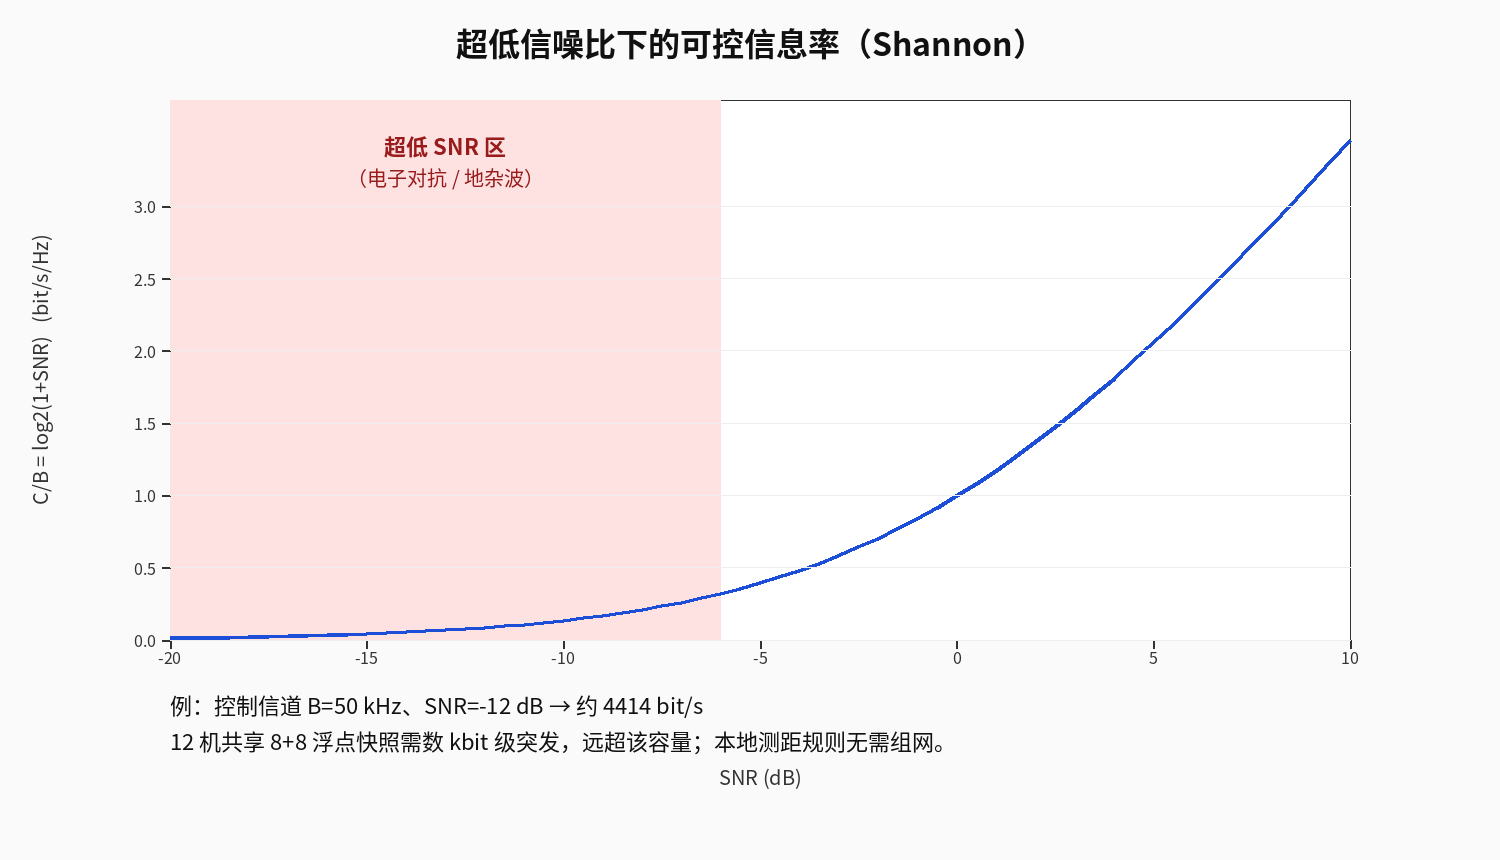
\includegraphics[width=0.92\textwidth]{figures/low_snr_capacity.png}
  \caption{超低信噪比区的归一化 Shannon 容量。红色区域对应电子对抗与地杂波下的典型工作点。}
  \label{fig:snr}
\end{figure}

\subsection{算力模组为什么不划算}

一次性弹药的预算恒等式是
\begin{equation}
  c_{\mathrm{shot}} = c_{\mathrm{airframe}} + c_{\mathrm{warhead}} + c_{\mathrm{seeker}} + c_{\mathrm{compute}}.
\end{equation}
$c_{\mathrm{airframe}}$ 与 $c_{\mathrm{warhead}}$ 已因消费电子下探；若 $c_{\mathrm{compute}}$ 达到数十至上百美元（含电源、屏蔽、散热），它会重新主导单价，却只服务一次前向推理。规则算法可在 Cortex-M 级 MCU 上以毫瓦功耗完成；网络即便量化到整数，仍需持续的矩阵单元与更大的 SRAM。图~\ref{fig:hw} 用本次实验的 ops 比作为量级锚点：规则侧按 MCU 计，网络侧按“专用小 NPU”的乐观下界计。真实视觉模型会把右侧柱再拉高。

\begin{figure}[H]
  \centering
  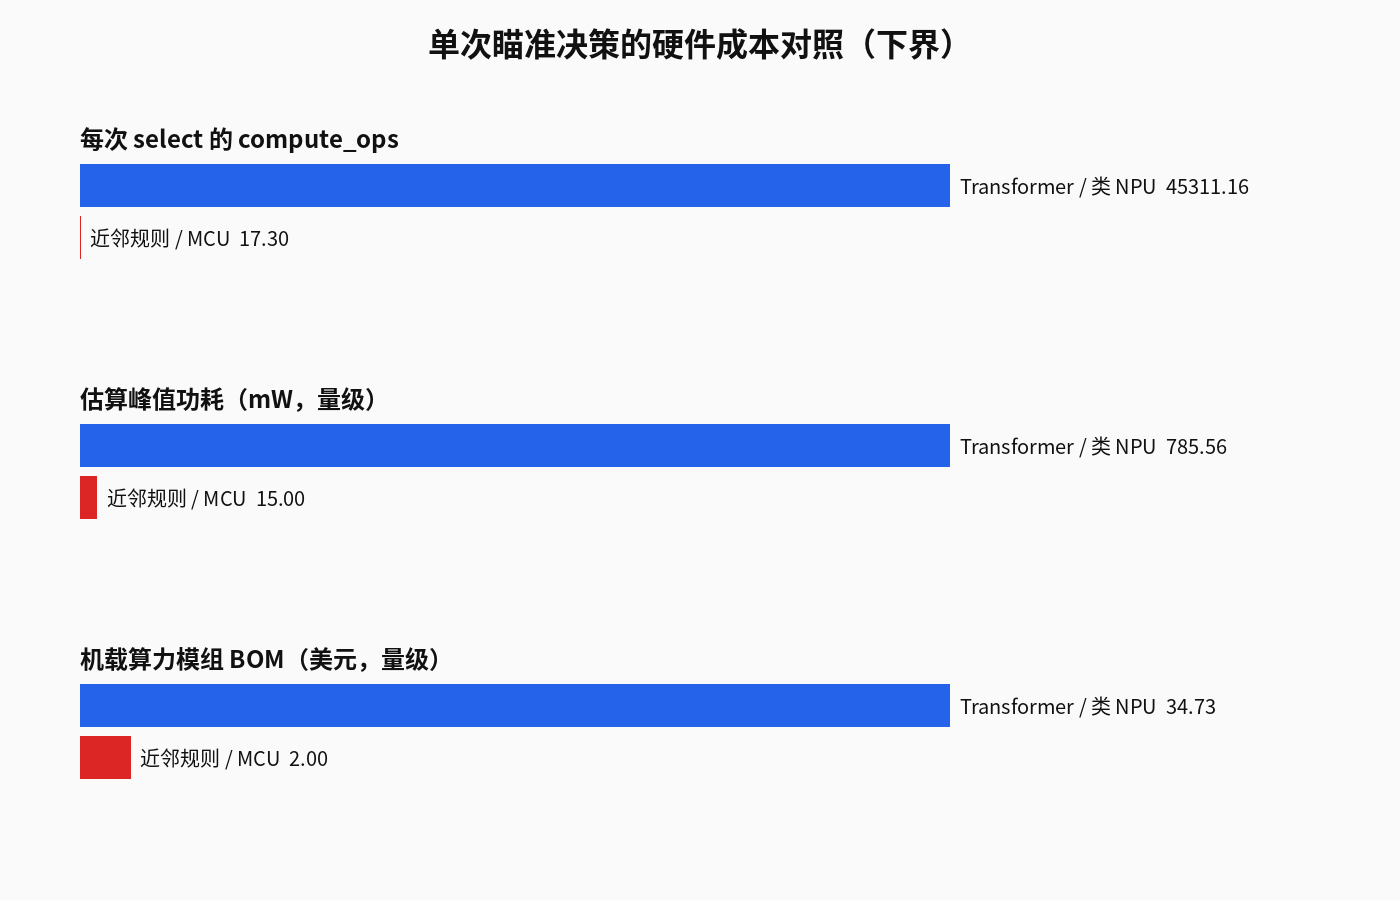
\includegraphics[width=0.92\textwidth]{figures/hardware_cost.png}
  \caption{单次瞄准的计算量、功耗与模组成本对照。网络柱为乐观下界。}
  \label{fig:hw}
\end{figure}

\section{实验设置}

\begin{table}[H]
\centering
\caption{默认仿真与评估协议}
\label{tab:setup}
\begin{tabular}{ll}
\toprule
项目 & 取值 \\
\midrule
圆半径 $R$ / 敌人数 & $200\,\mathrm{m}$ / 20 \\
编队 & 2 排 $\times$ 6，排距 $40\,\mathrm{m}$ \\
杀伤矩形 & $[-R,R]^2$，圆内切 \\
探测 $D$ / 航线间距 & $80\,\mathrm{m}$ / $80\,\mathrm{m}$（完美包含） \\
速度 / 步长 / $T_{\mathrm{kill}}$ & $25\,\mathrm{m/s}$ / $0.01\,\mathrm{s}$ / $0.05\,\mathrm{s}$ \\
消耗模型 & 命中即 \texttt{Expended}，无二次开火 \\
训练 & Transformer：8000 步合成 CE + 200 轮实装模仿 \\
训练损失 & 仅存活时间诱导的行为；\texttt{compute\_ops} 不进 loss \\
评估 & 两算法各 30 轮，种子 $20270823+i$ \\
评分 & $\overline{T}_{\mathrm{surv}}$（含 $T_{\mathrm{end}}$ 删失）、中和数、\texttt{compute\_ops} \\
\bottomrule
\end{tabular}
\end{table}

评估种子对两算法相同，因此地图实现是配对的：差异只来自决策。

\section{结果}

表~\ref{tab:res} 与图~\ref{fig:surv}--\ref{fig:kill} 汇总 30 轮配对评估。

\begin{table}[H]
\centering
\caption{30 轮同种子评估均值}
\label{tab:res}
\begin{tabular}{lccc}
\toprule
算法 & 场均中和数 & 平均存活时间 (s) & 每步 compute\_ops \\
\midrule
Transformer（对照） & 10.07 & 15.792 & $4.531\times 10^{4}$ \\
近邻涌现规则（研究） & 10.10 & 15.738 & $17.3$ \\
\midrule
规则相对网络 & $+0.03$ & $-0.054$ & $1/2619$ \\
\bottomrule
\end{tabular}
\end{table}

近邻规则在平均存活时间上略优（15.738 s 对 15.792 s），中和数几乎相同（10.10 对 10.07）。二者都远好于“全程弃权”的删失基线 $24\,\mathrm{s}$（路径长 600 m、速度 25 m/s）。

\subsection{高斯配对检验}

以同一种子的轮次为配对，令
\[
  \Delta_i = \overline{T}_{\mathrm{surv},i}^{\mathrm{(TF)}} - \overline{T}_{\mathrm{surv},i}^{\mathrm{(rule)}},
\]
并设 $\{\Delta_i\}$ 近似独立同分布于 $\mathcal{N}(\mu,\sigma^2)$。检验统计量
\[
  z = \frac{\bar\Delta}{s/\sqrt{n}},\qquad
  p_{\mathrm{two}} = 2\bigl(1-\Phi(|z|)\bigr),\qquad
  p_{\mathrm{one}} = 1-\Phi(z),
\]
其中 $\Phi$ 为标准正态 CDF，$p_{\mathrm{one}}$ 对应备择 $\mu>0$（规则使目标更早死亡）。等效性采用 TOST：在 $\delta=0.5\,\mathrm{s}$ 的实务无差异界下，检验 $H_0:|\mu|\ge\delta$。中和数作同样的配对 $z$ 检验。结果见表~\ref{tab:pval} 与图~\ref{fig:pval}。

\begin{table}[H]
\centering
\caption{30 轮配对高斯 $z$ 检验（$\Delta=$ Transformer $-$ 规则）}
\label{tab:pval}
\begin{tabular}{lcccc}
\toprule
指标 & $\bar\Delta$ & $z$ & 双侧 $p$ & 单侧 $p$（规则更优） \\
\midrule
平均存活时间 (s) & $+0.054$ & $1.178$ & $0.239$ & $0.119$ \\
中和数 & $-0.033$ & $-0.441$ & $0.659$ & --- \\
\midrule
存活时间 TOST $|\mu|<0.5\,\mathrm{s}$ & & & $p_{\mathrm{TOST}}<10^{-12}$ & 等效 \\
\bottomrule
\end{tabular}
\end{table}

双侧 $p=0.239$（存活）与 $p=0.659$（中和）均远大于 $0.05$，\textbf{不能拒绝两算法杀伤效能相同}。TOST 则在 $0.5\,\mathrm{s}$ 界内以极高把握接受等效：相对 $T_{\mathrm{end}}=24\,\mathrm{s}$，半秒的差异没有战术意义。点估计上规则更好：29/30 轮存活时间更低，28/30 轮中和数打平，单侧 $p=0.119$ 未达 $0.05$，故只将“更优”表述为方向一致的微小优势，而非显著优于网络。这正是装备论证所需要的形态——\textbf{简单规则与 Transformer 杀伤接近，并在点估计上略占优}，却少用约 2600 倍算力。

\begin{figure}[H]
  \centering
  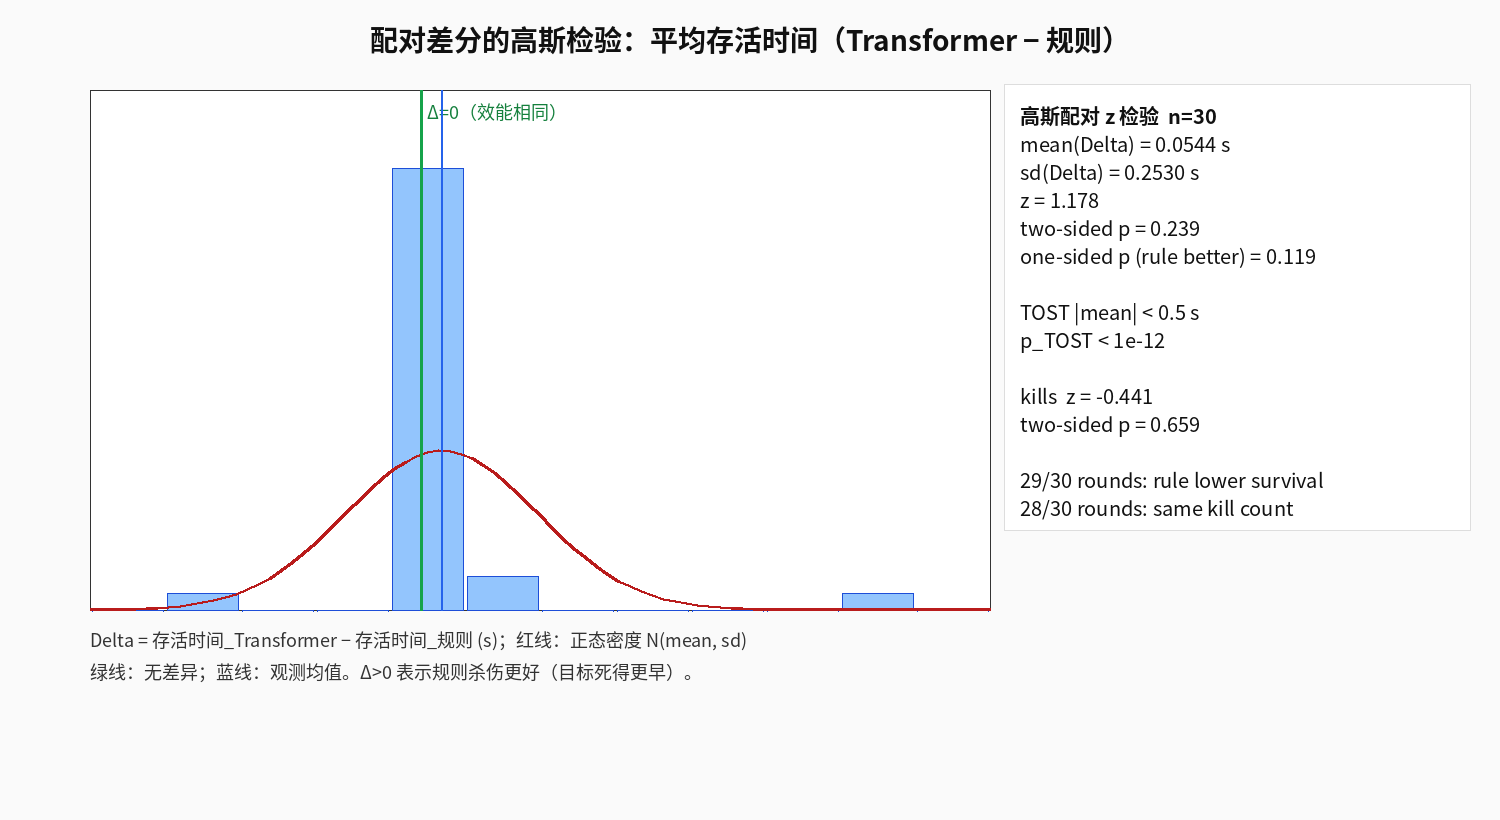
\includegraphics[width=0.92\textwidth]{figures/pvalue_gaussian.png}
  \caption{配对存活时间差分的直方图与拟合正态。绿线为无差异，蓝线为观测均值。$\Delta>0$ 表示规则更好。}
  \label{fig:pval}
\end{figure}

计算量则完全不在同一量级：规则每步约 17 次操作，网络约 45311 次，比值 2619；按每轮总 ops 计（$5.62\times 10^{8}$ 对 $2.12\times 10^{5}$）比值为 2647。该差距已经足够决定 MCU 与 NPU 的选型，而真实机载视觉网络只会把分母保持在 17、把分子再放大。

\begin{figure}[H]
  \centering
  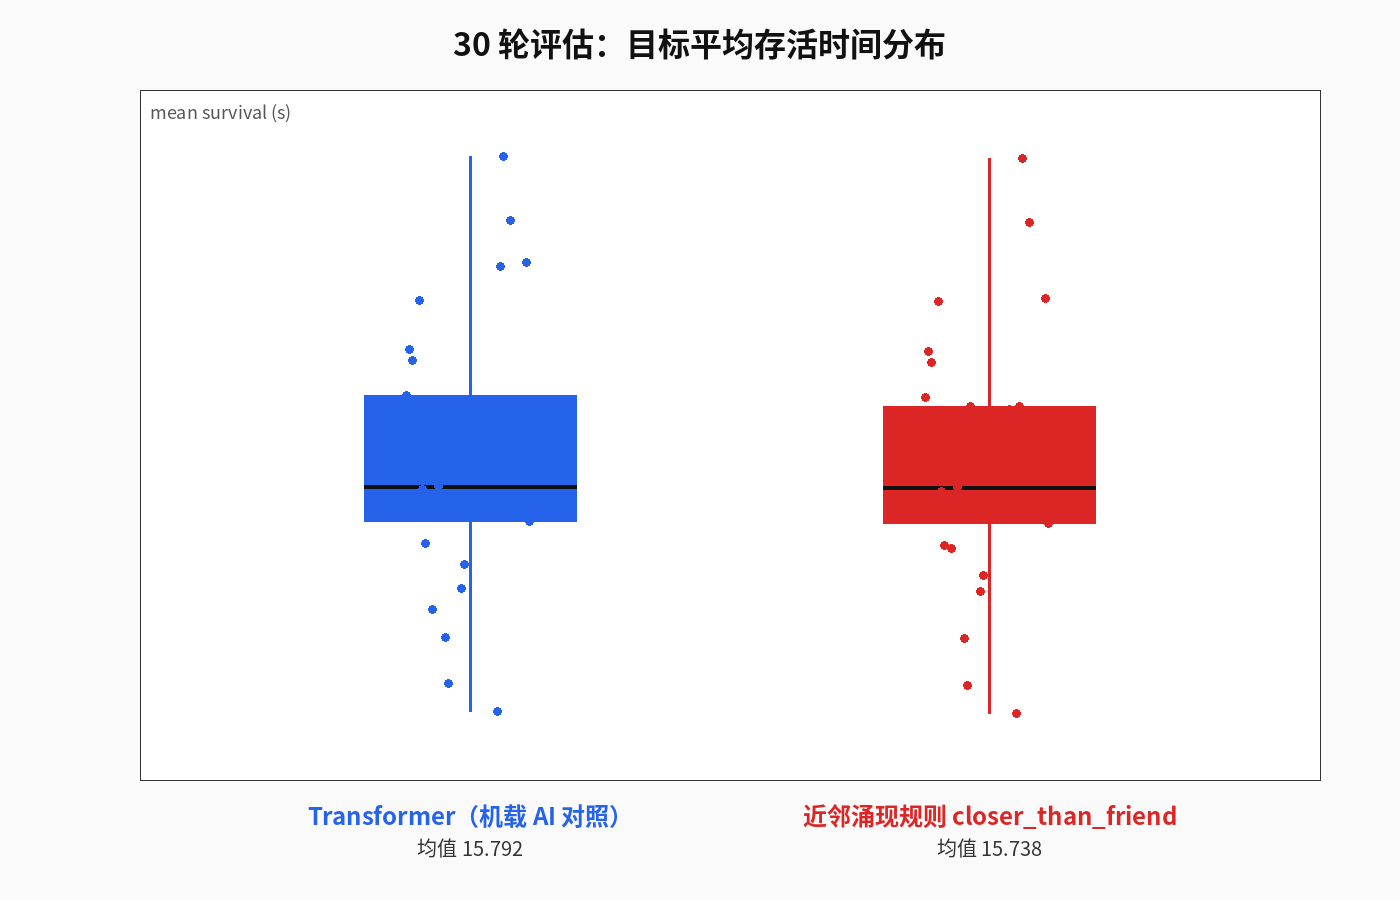
\includegraphics[width=0.92\textwidth]{figures/survival_compare.png}
  \caption{30 轮平均存活时间分布。越低越好；两算法中位与均值接近，规则略低。}
  \label{fig:surv}
\end{figure}

\begin{figure}[H]
  \centering
  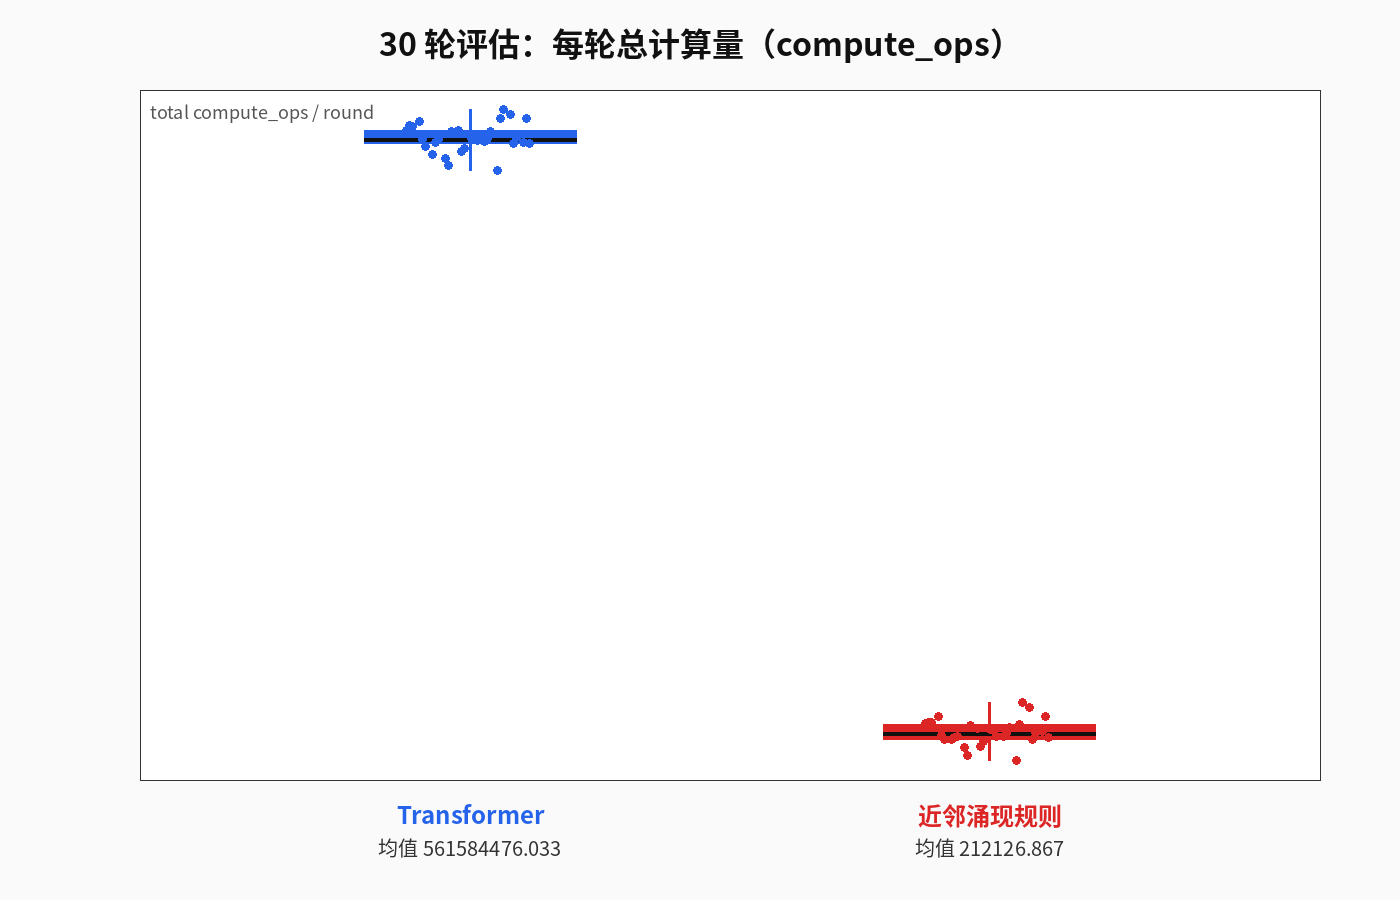
\includegraphics[width=0.92\textwidth]{figures/compute_ops_compare.png}
  \caption{30 轮每轮总 compute\_ops（对数纵轴）。网络比规则高三个数量级。}
  \label{fig:ops}
\end{figure}

\begin{figure}[H]
  \centering
  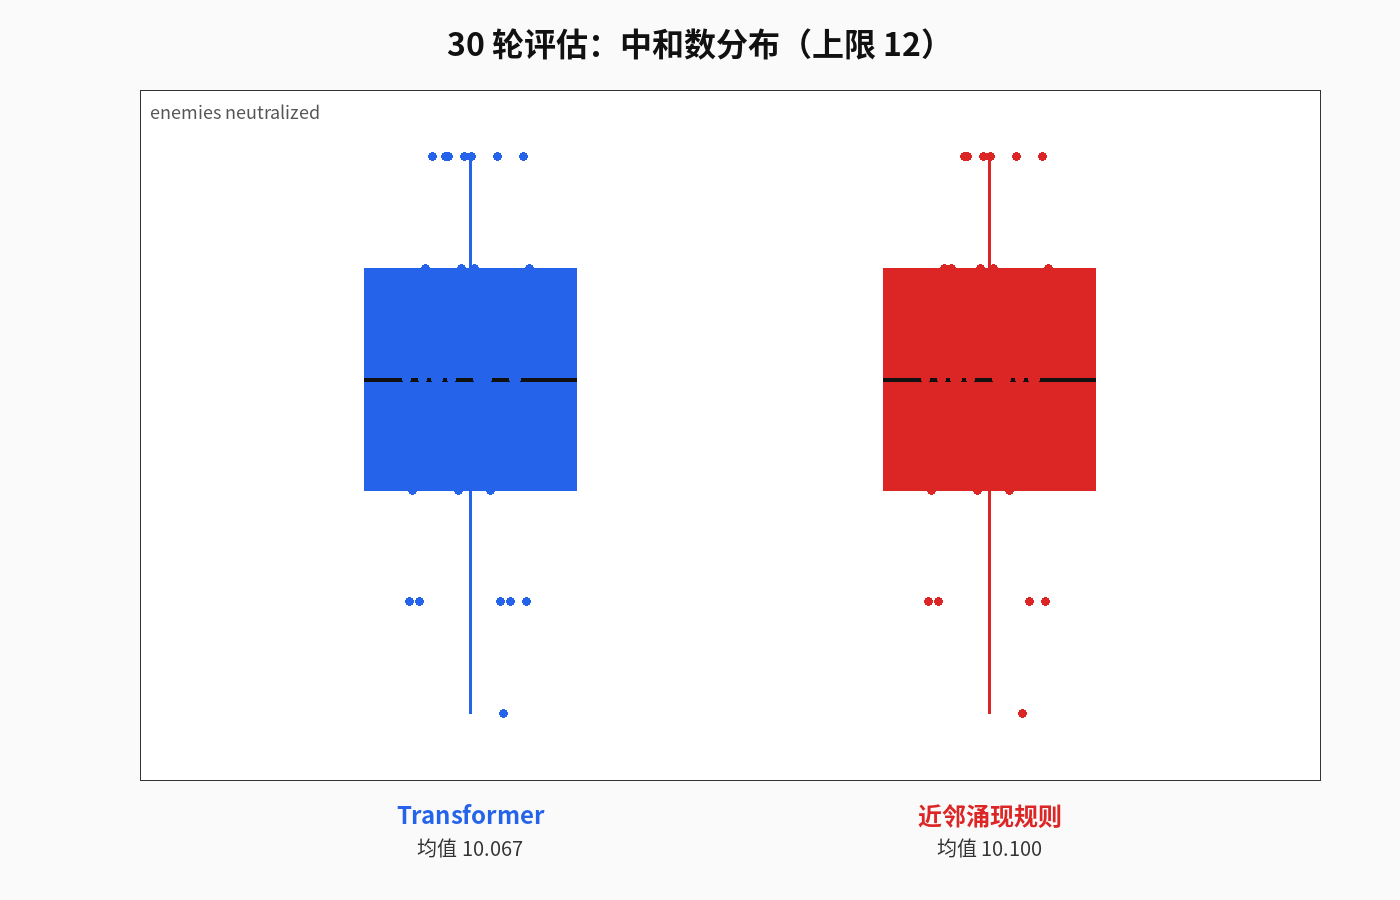
\includegraphics[width=0.92\textwidth]{figures/killed_compare.png}
  \caption{30 轮中和数分布。一次性模型上限为 12；两算法均稳定在约 10。}
  \label{fig:kill}
\end{figure}

需要强调：Transformer 并非“随机乱打”。训练轮次的场均中和在 8--12 之间，贪心评估亦达到 10.07，说明网络学会了“能打则打、友机更近则让”的合法策略。它只是没有\emph{超过}三行规则。把 2600 倍算力花在逼近一条最小值比较上，正是一次性平台不该做的事。

\section{讨论}

\subsection{涌现而不是规划}

近邻规则没有显式的“先导打南、后排打北”条款，但排距 $40\,\mathrm{m}$ 把该分工写进了不等式 $d_{\mathrm{tgt}}<d_{\mathrm{fr}}$。这是典型的形态—规则耦合：几何是协议。电子战环境下，协议若依赖无线电，会被 SNR 切断；若依赖相对位置，则与机体同在。只要编队还能飞，规则就还在。

\subsection{网络为什么没有赢}

可能原因有三。第一，8+8 快照的信息瓶颈：全局最优分配需要全图，本地窗口下近邻已接近充分统计。第二，一次性 12 弹使“打得更巧”的收益有上限，巧打与近打在扫掠几何下高度相关。第三，200 轮仿真对一层 Transformer 足以模仿规则，但不足以发现规则之外的稀疏战术——而那些战术若依赖机间约定，在超低 SNR 下也部署不了。

\subsection{对装备论证的含义}

若作战概念是“每人带若干架便宜 FPV，电子环境恶劣，打完即弃”，则经费应投向电池、战斗部、抗干扰遥控与传感器标定，而不是每机一块 NPU。机载 AI 更适合可回收侦察机或地面引导节点：那些平台能摊销算力，并能在较高 SNR 或有线回传下使用模型。把二者的成本结构互换，是范畴错误。

\subsection{局限}

仿真是二维匀速扫掠，敌方静止，探测为理想圆。真实 FPV 有姿态、风扰、图像识别虚警与飞手接管。这些因素对\emph{两种算法是共同的}：它们不改变“本地规则 vs 本地网络”的相对算力差，也不恢复超低 SNR 下的组网能力。若未来出现极低功耗、可忽略成本的模拟比较电路，规则仍可直接硬化；网络则仍需存储与乘加阵列。

\section{结论}

本文在杀伤区完美包含圆形战场的可复现平台上，对比了一次性 FPV 机群的两种本地瞄准算法。30 轮配对实验给出三点结论。

\begin{enumerate}
  \item \textbf{效能。} 近邻规则场均存活 15.74\,s、中和 10.10，Transformer 为 15.79\,s 与 10.07。高斯配对检验双侧 $p=0.239$（存活）与 $p=0.659$（中和），不能拒绝效能相同；TOST 在 $0.5\,\mathrm{s}$ 界内 $p<10^{-12}$，两者等效。点估计上规则略优（29/30 轮存活更低）。简单规则是有效的。
  \item \textbf{成本。} 规则每步约 17 ops，网络约 $4.53\times 10^{4}$ ops，相差约 2600 倍。一次性弹药不应为逼近一条比较式支付 NPU。
  \item \textbf{通信。} 超低 SNR 下有效信息的时延本身是稀缺品。两种算法都不依赖机间共享目标表；规则进一步把去冲突编码进编队几何，连“同步模型权重”都不需要。
\end{enumerate}

因此，在超低信噪比、一次性、低成本的 FPV 机群中，基于测距的简单涌现规则不仅是权宜之计，而且是与当前物理约束相匹配的主方案。给每架飞机安装 AI 大脑，既没有信道去喂它全局信息，也没有费效去证明那 2600 倍算力买到了额外的存活时间下降。

\section*{数据与可复现性}

源代码、训练权重、30 轮评估 CSV、SQLite 以及本论文的 \LaTeX/\textsc{pdf} 均公开发布于
\begin{center}
\url{https://github.com/1037104428/drones}
\end{center}
克隆后即可复现，无需访问作者本地路径：
\begin{verbatim}
git clone https://github.com/1037104428/drones.git
cd drones
cargo test
cargo run --release -- experiment \
  --train-rounds 200 --eval-rounds 30 --seed 20260823
\end{verbatim}
仓库中 \texttt{results/*.csv} 与 \texttt{data/experiment.sqlite} 为本文表~\ref{tab:res}--\ref{tab:pval} 的原始评估记录；\texttt{models/transformer.json} 为 200 轮训练后的权重。同一种子重复评估时，中和结果与 \texttt{compute\_ops} 逐行一致。问题与讨论请走 GitHub Issues。

\begin{thebibliography}{9}

\bibitem{shannon1948}
C.~E. Shannon.
\newblock A mathematical theory of communication.
\newblock {\em Bell System Technical Journal}, 27:379--423, 623--656, 1948.

\bibitem{sklar2001}
B.~Sklar.
\newblock {\em Digital Communications: Fundamentals and Applications}.
\newblock Prentice Hall PTR, Upper Saddle River, NJ, 2nd edition, 2001.

\bibitem{reynolds1987}
C.~W. Reynolds.
\newblock Flocks, herds, and schools: A distributed behavioral model.
\newblock {\em Computer Graphics (SIGGRAPH '87 Proceedings)}, 21(4):25--34, 1987.

\bibitem{camazine2001}
S.~Camazine, J.-L. Deneubourg, N.~R. Franks, J.~Sneyd, G.~Theraulaz, and E.~Bonabeau.
\newblock {\em Self-Organization in Biological Systems}.
\newblock Princeton University Press, 2001.

\bibitem{vaswani2017}
A.~Vaswani, N.~Shazeer, N.~Parmar, J.~Uszkoreit, L.~Jones, A.~N. Gomez, L.~Kaiser, and I.~Polosukhin.
\newblock Attention is all you need.
\newblock In {\em Advances in Neural Information Processing Systems 30} (NIPS 2017), 2017.

\end{thebibliography}

\end{document}
